\subsection{Applying Sampling Methodologies to the Nugget Framework and Validating the Selected Samples (Goals 2 \& 3)}
\label{sec:sampling_methodology_validation}

The primary objective of Nugget is to support diverse sample selection methodologies while providing efficient interval analysis, binary-independent samples, and scalable validation capabilities.
In this section, we leverage these features to execute the selected samples, \emph{nuggets}, directly on real hardware, enabling us to assess whether different sampling strategies can accurately predict full workload performance \emph{without relying on simulation}.

Because this thesis does not propose new sampling algorithms, we focus on two straightforward approaches: random sampling and LLVM IRBB vector-based k-means clustering.
We show that Nugget seamlessly implements these methodologies and facilitates validating the selected samples on \emph{real hardware}.
We also show that different workloads may benefit from different sampling strategies; Nugget enables discovering and applying methods tailored to specific workload characteristics.
Moreover, we highlight the importance of validating sampling methodologies across multiple machines, especially when the target system is not yet available.
Finally, we discuss the overhead introduced by the hooks used to mark sample intervals within nuggets.

\subsubsection{Sampling Methodologies}
\label{sec:sampling_methodology}

For the random sampling approach, we randomly select a set of intervals from the program execution to estimate its average or cumulative properties.
This selection method is based on statistical sampling methods~\cite{smarts}.

For the clustering approach, we use the k-means algorithm to cluster the IRBB vectors, select ``k'' samples to represent the program phases of the workload, and use the cluster weights to estimate the average or cumulative properties of the program execution.
This approach is based on basic block vector (BBV) phase-identification techniques~\cite{survey_phase_classification} (e.g., SimPoint) and on the fact that the IRBB vector is an abstraction of the actual BBV.

We refer to the random approach as ``Random'' and the clustering approach as ``K-means''.
We use 50 samples as the target number for both methodologies, which is statistically large enough to approximate the population distribution~\cite{hogg2020psi}.
We apply the Silhouette score with the K-means algorithm to determine the optimal number of clusters for each workload, enforcing the constraint $\#\text{clusters} \le 50$ (with $k = 50$ as the upper bound).
We assign equal weights to all intervals in the ``Random'' approach, whereas the ``K-means'' approach weighs each interval according to the size of its cluster.

\subsubsection{Sample Validation}
\label{sec:sample_validation}

\FloatBarrier
\begin{figure*}[!t]
    \centering
    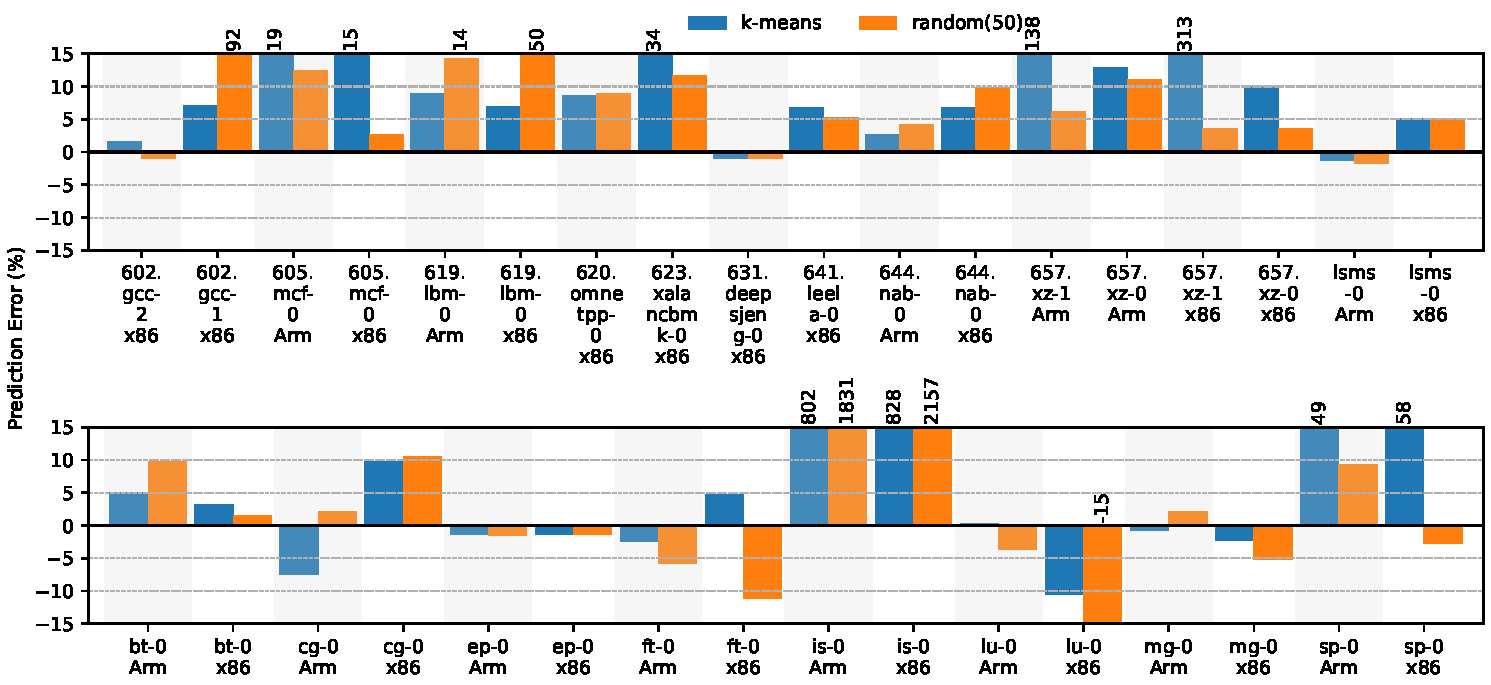
\includegraphics[width=\textwidth]{images/prediction_error_by_machine_method_2panel.pdf}
      \caption{
        Prediction error by machine and sampling method.
        \textbf{All results shown are obtained from executing the nuggets directly on real hardware}, without using simulation.
    }
    \label{fig:prediction_error_by_machine_method}
\end{figure*}

We use the analysis information collected in Section~\ref{sec:mix_of_workload_types} to select samples with the ``Random'' and ``K-means'' approaches.
We then generate nuggets for the selected samples and validate them as described in the Sample Creation and Validation step in Figure~\ref{fig:nugget_pipeline}.
The nuggets are used to predict the runtime of each workload, with the runtime of the full execution serving as the baseline for calculating prediction error.
We choose runtime as the metric because it is a common target of sampling methodologies~\cite{looppoint}, and IPC has been shown to be unsuitable for multi-threaded workloads~\cite{ipc_considered_harmful}.

Figure~\ref{fig:prediction_error_by_machine_method} presents the prediction errors of nuggets generated by the Random and K-means approaches for each workload on the real-hardware machines listed in Table~\ref{tab:system-configuration}. 
As shown, many workloads exhibit significant errors, often exceeding the accuracy reported by prior methodologies such as SimPoint (3\% for single-threaded workloads) and LoopPoint (2.9\% for 8-threaded workloads).

Several factors contribute to these elevated errors.
(1) The sampling methodologies are naively designed. For example, the Random approach relies heavily on luck and the specific composition of the interval pool.
(2) Previous work rarely validates samples on real hardware~\cite{wavelet-based,taskpoint,simpoint,looppoint,smarts,fsa,cross_binary_simpoints,pacsim,barrier_point,simpoint-plus,parrot}.
Instead, they mostly rely on user-mode-only simulation, which is typically less noisy due to more controllable thread interleaving compared to actual hardware~\cite{variability_in_architectural_simulations_of_multithreaded_workloads,11_gem5,survey-simulator-techniques,deterministic_shared_memory_multiprocessing}. 
In Section~\ref{sec:model_performance_evaluation}, we further analyze the sources of prediction error using smaller workloads in simulation.
(3) Prior work rarely validates large workloads as we used in our experiments (e.g., reference input sizes for CPU2017). 
Larger and more realistic applications exhibit increasingly complex behaviors~\cite{characterizing_and_comparing_prevailing_simulation_techniques,hot-region-spec2017, simpoint,spec2017-workload-characterization,wavelet-based,looppoint}, which demand more representative sample sets, as discussed in Section~\ref{sec:validating_the_selected_samples_is_infeasible}.
In such cases, large program phases can amplify prediction error.
(4) Hardware-based nuggets incur additional overhead for the begin and end interval markers, particularly in multi-threaded contexts, which further inflates prediction error. We provide a detailed discussion of this overhead in Section~\ref{sec:hook_overhead}.


As the figure shows, the sampling approach that yields the lowest prediction error varies by workload.
For example, for ``sp,'' the ``Random'' approach with 50 samples achieves the lowest prediction error across all methods, and this holds on both machines, suggesting that this sample set is architecturally and microarchitecturally independent.
In contrast, for ``lbm,'' the ``K-means'' approach consistently yields the lowest prediction error.

\begin{figure}[!t]
    \centering
    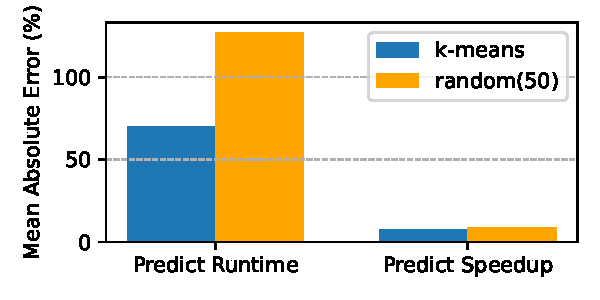
\includegraphics[width=\linewidth]{images/speedup_vs_runtime_prediction_error.pdf}
    \caption{Comparison of average absolute runtime prediction error and speedup prediction error for the nuggets shown in Figure~\ref{fig:prediction_error_by_machine_method}. Speedup is computed as the ratio of predicted runtimes between two machines.}
    \label{fig:speedup_vs_runtime_error}
\end{figure}

Although the absolute runtime prediction errors can be large for some workloads, a more practically relevant question is whether these errors are consistent across machines.
To investigate this, we use the predicted runtimes from our nuggets to compute predicted speedup between the two hardware platforms and compare the resulting speedup prediction error against the individual runtime prediction errors.
Figure~\ref{fig:speedup_vs_runtime_error} presents this comparison.
As shown, the average speedup prediction error is significantly smaller than the average runtime prediction error, even when the outlier workload ``is'' is included in the data set.
For example, the K-means approach yields an average runtime prediction error of 70.13\% but a speedup prediction error of only 7.58\%, while the Random approach with 50 samples yields 126.90\% for runtime but only 8.92\% for speedup.
This occurs because when the prediction error is consistent across machines---that is, the predicted runtime on both machines deviates from the true runtime in the same direction and by a similar proportion---the errors cancel out in the speedup ratio, yielding an accurate relative performance prediction.
This observation indicates that \emph{consistency} of prediction error across platforms matters more than minimizing the absolute prediction error on any single machine.

We focus on demonstrating Nugget's ability to validate samples on distinct machines in this section.
In Section~\ref{sec:model_performance_evaluation}, we will further analyze how to utilize the hardware validation data with a case study.
We also find that maintaining consistency across machines is a stronger indicator of sample quality than minimizing prediction error on any single platform.
This insight further underscores the importance of efficient, cross-platform validation in the design of robust sampling methodologies.

\subsubsection{Hook Overhead}
\label{sec:hook_overhead}

\begin{figure}[!t]
    \centering
    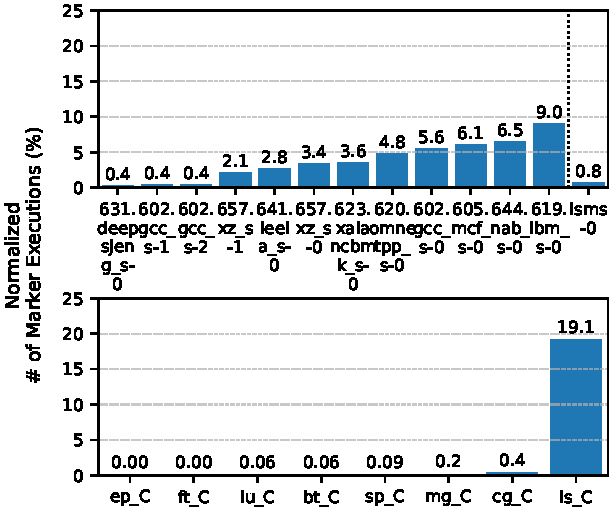
\includegraphics[width=\linewidth]{images/marker_executions_2panel.pdf}
    \caption{The number of marker hook executions for the randomly selected nuggets shown in Figure~\ref{fig:prediction_error_by_machine_method}. The number of hook executions is normalized to the total number of IRBB executions during all nugget executions for each workload and input pair.}
    \label{fig:marker_executions_combined}
\end{figure}

Nugget uses hook instructions to mark sample intervals, which can introduce runtime overhead during workload execution.
In Figure~\ref{fig:marker_executions_combined}, we present the number of times the marker hooks are executed for the randomly selected nuggets shown in Figure~\ref{fig:prediction_error_by_machine_method}.
The number of hook executions is normalized to the total number of IRBB executions during all nugget executions for each workload and input pair.
As shown, ``is'' exhibits a significantly higher number of hook executions compared to other workloads, indicating that the prediction error observed for ``is'' in Figure~\ref{fig:prediction_error_by_machine_method} is influenced by the excessive overhead from hook executions.
Because ``is'' frequently executes only a small number of IRBBs within a parallel region, it triggers an excessive number of hook invocations.
``is'' was also one of the workloads with the largest overheads for analysis as shown in Figure~\ref{fig:simulation_interval_analysis_overhead}.
This leads to substantial overhead and results in inaccurate prediction errors.
Hook overhead can only slow execution, so it can cause false negatives (rejecting good samples) but is unlikely to cause false-positive conclusions.

For other workloads, the number of hook executions does not show a clear correlation with the prediction error observed in Figure~\ref{fig:prediction_error_by_machine_method}.
Cleanly separating the impact of hook overhead from other sources of prediction error is still challenging.
The number of hook executions and the prediction errors observed suggest that the cutoff line for a good marker should be executing lower than 10\% for single-threaded workloads and lower than 1\% for multi-threaded workloads, in terms of the total IRBBs executed in the nugget, to avoid significant overhead impacting the validation results.
Multi-threaded workloads are more sensitive to hook overhead due to the synchronization required for counting and threshold checks, as discussed in Section~\ref{sec:overhead_of_hooks}.

This behavior highlights a limitation of the current hook-based interval marking approach.
Future work could explore alternative mechanisms to reduce this overhead or to decouple it from the validation results.
However, addressing this issue is nontrivial, especially for multi-threaded workloads: overhead in parallel regions can differ significantly from that in serial regions, and parallelism may sometimes mask or amplify hook-related costs, complicating the isolation of their impact.

It is important to note that this overhead is unique to real hardware execution.
In simulation, as discussed in Section~\ref{sec:overhead_of_hooks}, sample intervals can be marked directly by the simulator without introducing runtime overhead.
